%!TEX encoding = UTF-8 Unicode
\documentclass[ % options,
    a4paper,    % papersize
%    cjk,       % for cjk-ko
%    usedotemph,% for cjk-ko's \dotemph
    amsmath,    % load amsmath.sty to typeset math materials
    itemph,     % to disable gremph default (xe/lua)
%    footnote,  % korean style footnote
%    chapter,   % to use \chapter
11pt]{oblivoir}     % xoblivoir and oblivoir are identical.

\ifPDFTeX       % latex, pdflatex
%    \usepackage{newtxtext}    % Latin fonts
\else\ifLuaOrXeTeX   % xelatex or lualatex
%  \setmainfont[Ligatures=TeX]{TeX Gyre Termes}   %% Latin fonts
  \defaultfontfeatures{Ligatures=TeX}
  \setkormainfont(* ExtraBold)(*){NanumMyeongjo}(* Bold)(*){HCR Batang}
  \setkorsansfont{NanumGothic}
  \setkormonofont[Scale=.95]{NanumGothic}
\fi\fi

\usepackage{unicode-math}
%\setmathfont{XITS Math}
\usepackage{ulem}
\usepackage[numbers, square]{natbib}
\usepackage{tabu}
\usepackage{caption}
%
% page layout
%
\setlrmarginsandblock{*}{1in}{*}
\setulmarginsandblock{*}{1in}{1.1}
\checkandfixthelayout
%

\begin{document}

\begin{center}
\Large{\textbf{참고 논문 정리}}
\end{center}


\begin{flushright}
\textit{방송통신대학원 정보과학과 김호현} \\
\end{flushright}
\vspace{-5mm}
\noindent\rule{\textwidth}{.5pt}

\vspace{-5mm}
\section{A moving-average-filter-based hybrid ARIMA-ANN model for forecasting time series data\cite{babu2014}}

\begin{description}\tightlist
\item[저자] C.N.Babbu, B.E.Reddy
\item[학술지] Applied Soft Computing 2014(23), 27--38
\end{description}

\subsection{연구배경 및 목적}
선형 및 비선형의 결합 모델은 선형 혹은 비선형 모델을 각각 적용하는 것 보다 더 좋은 예측력을 보인다.  지금까지 여러가지 Hybrid ARIMA-ANN 모델이 있었으나 더욱 개선 여지가 있다.  

\subsection{연구방법}

2절에 ARIMA, ANN, Zhang's hybrid ARIMA-ANN, Khashei and Bijari's hybrid ARIMA-ANN 과 자신의 제안 모델인 MA 필터 hybrid ARIMA-ANN을 비교하였다.

\begin{enumerate}
\item Zhang's hybrid ARIMA-ANN 모델

Time series data는 선형과 비선형 분분의 합이라고 가정한다. 먼저 ARIMA 모델을 세워 예측을 하고 난 후, error 시퀀스를 ANN을 이용하여 예측한 후 이 둘을 합하는 방식이다.

\item Khashei abd Bijari's hybrid ARIMA-ANN 모델

이 방법 역시 Time series data는 선형과 비선형 부분의 합계라고 가정한다. 먼저 ARIMA 모델을 세워 예측을 하여 error 시퀀스를 구한 후, 원 과거 데이터와 error 데이터를 ANN에 입력하여 예측하는 방식이다.

\item Proposed hybrid ARIMA-ANN 모델

원 시계열 데이터에 이동평균 필터를 사용하여 추세 데이터와 잔여 데이터로 분리한다. 추세 요소는 변동성이 작으며(low volatility), 잔여요소는 변동성이 높다(high volatility).
추세 요소는 ARIMA 모델을 세워 예측하고, 잔여요소는 ANN으로 예측을 한 후, 이 둘을 합하여 최종 결과를 얻는다.
\end{enumerate}

\subsection{실험 자료}
3절에 실험 결과를 제시하였다. 측정치로는 MAE, MSE를 사용하였다.

\begin{enumerate}\tightlist
\item Simulated data set (총 100개, 예측에 30개) -- AR(2,0,0), ANN 2x2x1
\item Sunspot data (1700-1987, 288개)-- MA length: 37, ARIMA(9,0,0),
\item Electricity price data (2013.5, 총744개, 24개/168개를 예측에 사용) -- MA length: 25, ARIMA(1,1,1)
\item Stock market data (L\&T 종가 200거래일, 20를 예측에 사용) -- MA length: 90
\end{enumerate}

\subsection{결론}
변동성이 낮은 선형관계는 ARIMA가, 변동성이 높은 비선형관계는 ANN이 담당하는 Proposed 모델의 예측력이 가장 높았다. 예측력이 좋은 순서는 Proposed -- Khashei and Bijari -- Zhang -- ANN - ARIMA 이었다.


\section{An artificial neural network (p, d, q) model for timeseries forecasting\cite{khashei2010}}

\begin{description}\tightlist
\item[저자] Mehdi Khashei, Mehdi Bijari
\item[학술지] Expert Systems with applications 37 (2010) 479-489
\end{description}

\subsection{연구배경 및 목적}
ANN은 다양한 time series 데이터의 예측에 적용 가능하지만 정확성에 있어 만족할 수준이 아니다. 서로 판이하게 다른 모델을 결합하는 방법은 정확성을 향상시킨다는 이론적, 경험적으로 알려져 있다.  이 논문에서 ANN의 예측력을 높이기 위해 ARMIA와 결합(ARIMA로 데이터를 사전처리)하는 hybrid 모델을 제안한다.

\subsection{연구방법}
 서론에서 ANN의 장점과, 타 모델과의 결합을 통해 예측력이 좋아진다는 것이 이론적, 경험적으로 알려져 있다고 언급.

2절에서는 ANN, ARIMA을 설명하고, 3절에서는 제안모델의 방법을 제시하고
4절에서는 비교실험을 하였다.

\begin{enumerate}\tightlist
\item Zhang's hybrid ARIMA-ANN 모델
\item Khashei abd Bijari's hybrid ARIMA-ANN 모델
\item Proposed hybrid ARIMA-ANN 모델
\end{enumerate}


\subsection{실험 자료}

\begin{enumerate}\tightlist
\item Wolf's Sunspot data (1700-1987, 288개) 

  Training: 221(1700-1920), Test: 67(1921-1987),  AR(9,0,0), ANN 8x3x1

\item Canadian lynx data (1821-1934, 114개) -- AR(12,0,0), ANN 8x4x1

  Test: last 14 years

\item British pound/US dollar exchange data (1980-1993, 731개) -- ARIMA: random walk ($y_t= y_{t-1} + \varepsilon_t$), ANN 12x4x1
\end{enumerate}


\subsection{결론}
ARIMA 모델로 예측을 하여 error 시퀀스를 구한 후, 원 과거 데이터와 error 데이터를 ANN에 입력하는 hybrid 방법은 기존의 방법들을 능가하는 정확성을 보인다.
 

\section{Time series forcasting using a hybrid ARIMA and neural network model\cite{zhang2003}}

\begin{description}\tightlist
\item[저자] G.P.Zhang
\item[학술지] Neurocomputing 50 (2003) 159-175
\end{description}

\subsection{연구배경 및 목적}
시계열 예측에 ARIMA 모델이 광범위하게 사용되어 왔다. ARIMA 모델을 데이터 간의 선형관계는 잘 나타낼 수 있으나, 비선형 패턴은 처리할 수 없기 때문에 실세계의 문제에 ARIMA를 적용 시 만족할 만한 결과를 얻지 못한다. 최근 ANN을 시계열 예측 문제에 적용하려는 연구가 활발한데, ANN은 비선형 모델링 능력을 갖고 있다는 장점이 있다. 본 연구에서는 이 둘의 장점을 결합한 혼합 모델을 제안한다.

\subsection{연구방법}

2절에 시계열 예측 모델을 ARIMA 모델, ANN 접근법을 설명하였다. 3절에 hybrid 방법론을 설명하였다.


\begin{enumerate}\tightlist
\item ARIMA 모델을 수립하여 선형관계를 분석한다.
\item ARIMA에서 얻어진 residual을 ANN에 넣어 비선형 관계를 학습하여 결과를 얻는다.
\item 상기 둘의 결과를 더한다.
\end{enumerate}

4절에서는 ARIMA, ANN, Hybrid를 적용한 실험결과를 비교하였다. 측정값으로는 MSE, MAE(MAD)를 사용하였다.

\subsection{실험 자료}
\begin{enumerate}\tightlist
\item Sunspot data (1700-1987, 288개) -- AR(9,0,0), ANN 4x4x1
\item Canadian lynx data (1821-1934, 114개) -- AR(12,0,0), ANN 7x5x1
\item British pound/US dollar exchange data (1988-1993, 731개) -- ARIMA: random walk ($y_t= y_{t-1} + \varepsilon_t$), ANN 6x6x1
\end{enumerate}

\subsection{결론}

ARIMA와 ANN의 장점을 결합한 hybrid 모델은 각각을 독립적으로 사용했을 때 보다 더 좋은 결과를 보인다.


\section{Understanding LSTM Networks\cite{lstmblog}}

\begin{description}\tightlist
\item[출처] colah's blog 
\item[학술지] http://colah.github.io/posts/2015-08-Understanding-LSTMs/
\end{description}

\subsection{Recurrent Neural Networks}
전통적인 FFNN은 데이터의 순서를 기억하지 못한다. 따라서 앞뒤 관계가 중요한 경우 잘 학습할 수 없다. RNN은 이 문제를 해결하려는 것이다.  과거의 문맥을 기억할 수 있는 능력을 가지고 있다.

\hfil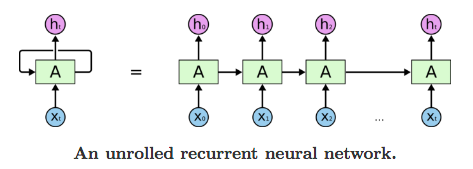
\includegraphics[width=.7\textwidth]{rnn1.png}\hfil
\begin{align}
h_t &= H(W_{xh}x_t - W_{hh}h_{t-1} + b_h)\\
y_t &= W_{hy}h_t+ b_y
\end{align}

\subsection{Problem of Long Term Dependencies}
그러나 표준 RNN은 입력과 출력 간의 간격이 멀어지면 문제가 발생한다.

\hfil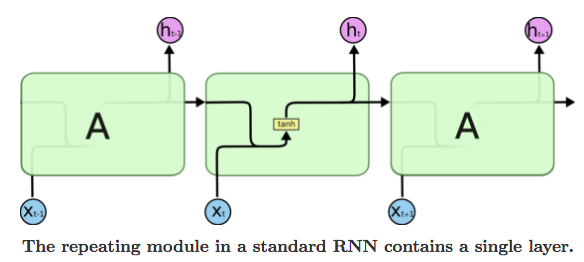
\includegraphics[width=.7\textwidth]{rnn3.png}\hfil

\hfil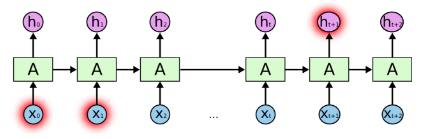
\includegraphics[width=.7\textwidth]{rnn2.png}\hfil

\subsection{Long Short Term Memory - LSTM}
단순 RNN은 vanishing gradient 문제를 가지고 있어, 긴 문맥을 기억할 수 없다는 문제가 있다. 최근 음성인식, 자연어 처리, 이미지 capationing 등에서 눈부신 성과를 내고 있는 RNN은 거의 대부분이 LSTM을 이용한 것으로, LSTM은 Vanishing gradient 문제를 해결하였다.

\hfil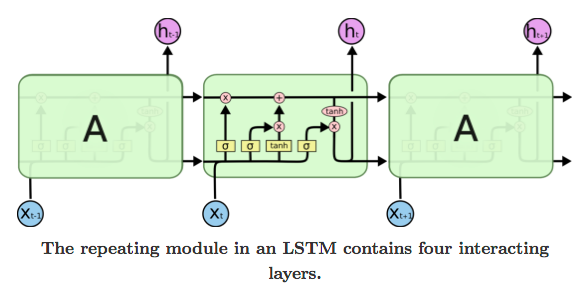
\includegraphics[width=.9\textwidth]{lstm1.png}\hfil
\begin{align} 
i_t &= \sigma(W_{xi}x_t + W_{hi}h_{t-1} + W_{ci}c_{t-1} + b_i) \\
f_t &= \sigma(W_{xf}x_t + W_{hf}h_{t-1} + W_{cf}c_{t-1} + b_f) \\
c_t &= f_tc_{t-1} + i_ttanh(W_{xc}x_t + W_{hc}h_{t-1} + b_c) \\
o_t &= \sigma(W_{xo}x_t + W_{ho}h_{t-1} + W_{co}c_t + b_o) \\
h_t &= o_ttanh(c_t)
\end{align}


\subsection{Gated Recurrent Unit - GRU}
여러가지 LSTM의 변형이 존재하며, 그 중 대표적인 것이 GRU이다.

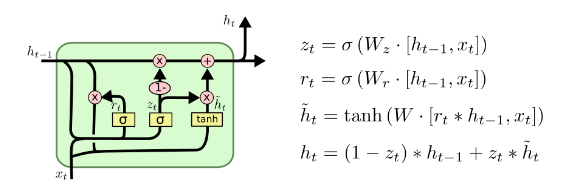
\includegraphics[width=.9\textwidth]{gru.png}


\subsection{결론}
최근 RNN의 눈부신 성과의 배경에는 LSTM이 있다. LSTM은 Vanishing gradient 문제를 해결하였다.  시계열 데이터는 시간 순서대로 발생하는 데이터로 앞의 데이터가 뒤의 데이터에 영향을 주므로 RNN을 적용하는 것이 자연스러운 일이다.

RNN에 LSTM을 적용함으로써 기존의 ANN 및 Hybrid ANN을 뛰어넘는 예측 모델 수립이 가능할 것으로 생각된다.


\section{Speech Recognition with deep recurrent neural networks\cite{graves2013}}

\begin{description}\tightlist
\item[저자] Graves, Alex and Mohamed, Abdel-rahman and Hinton, Geoffrey
\item[학술지] 2013 IEEE international conference on acoustics, speech and signal processing
\end{description}

\subsection{연구배경 및 목적}
긴 범위의 문맥을 기억할 수 있는 RNN과, data의 다층 표현을 가능케 하는 다층 구조를 결합한 deep recurrent neural networks를 음성인식에 적용하고자 하였다.

음성은 한 번에 기록되므로 후속음이 전음에 미치는 영향도 활용하기 위해 양방향 RNN을 이용한다. 

\subsection{연구방법}
2절에 Recurrent Neural Networks와 LSTM Cell을 수식을 들어 설명하고 있으며, 
LSTM 셀과 양방향 RNN의 그림을 싣고 있다.

\hfil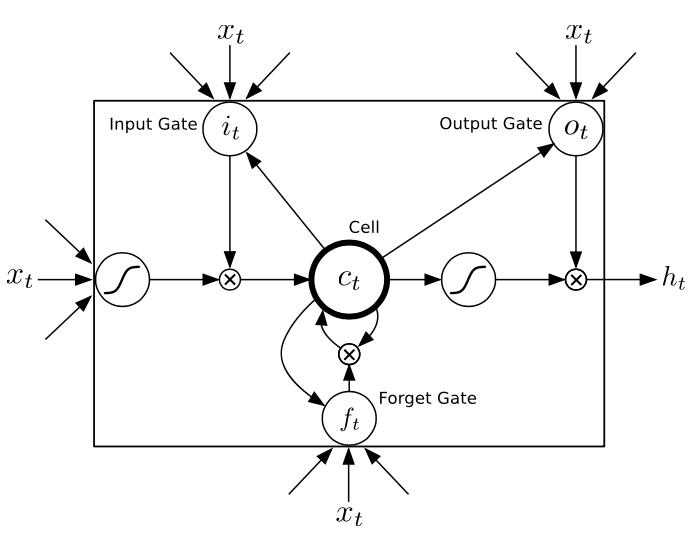
\includegraphics[width=.7\textwidth]{lstm2.png}\hfil

\hfil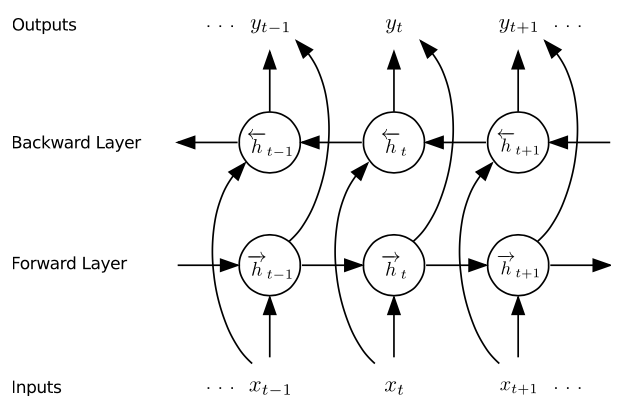
\includegraphics[width=.7\textwidth]{bi-rnn.png}\hfil

\subsection{실험방법}
TIMIT Corpus에 대해 depth와 layer size를 서로 다르게 하여 9가지 구조의 RNN을 만들어 비교 실험하였다.

\subsection{결론}
실험결과 depth가 layer size 보다 더 중요하다는 사실을 알았다. (이것은 Deep networks에 대한 과거의 연구와 일치한다.)

Deep, bidirectional, LSTM Recurrent Neural Networks를 통해 음소인식에서 지금까지 최고의 성능을 얻을 수 있었다.


\section{rnn : Recurrent Library for Torch7\cite{leonard2015}}

\begin{description}\tightlist
\item[저자] Leonard, Nicholas and Waghmare, Sagar and Wang, Yang
\item[학술지] arXiv preprint arXiv:1511.07889
\end{description}

\subsection{참고 사항}
simple RNN, LSTM RNN 등을 쉽게 구현할 수 있도록 하는 Torch RNN package.
Sequencer, Recurrence 사용법.
LSTM implementation 수식


\bibliographystyle{plainnat}
\bibliography{references}

\end{document}

